\documentclass[12pt]{article}

% Packages
\usepackage[utf8]{inputenc}
\usepackage{amsmath}
\usepackage{graphicx}
\usepackage{hyperref}
\usepackage{geometry}
\usepackage{setspace}
\usepackage{caption}
\usepackage{subcaption}
\usepackage{tikz}
\usepackage{listings}
\usepackage{xcolor}
\usepackage{pgfplots}
\usepackage{pgfplotstable}
\usepackage{amssymb}
\pgfplotsset{compat=newest}

\definecolor{darkgreen}{rgb}{0.0, 0.5, 0.0} % Darker green color

% Page Setup
\geometry{a4paper, margin=1in}
\setstretch{1.5}

% Title and Author
\title{Diagnosis, Treatment, and Imaging Analysis Performed by Machine Learning Approaches}
\author{Emilio Daza}
\date{\today}

\begin{document}

% Title Page
\maketitle

\section{Methodology}
\subsection*{Neural Network for Diagnosis}

\indent The model is composed of \textbf{5} layers and \textbf{113} neurons in total (post input layer). The number of layers and neurons is totally adjustable by the user to maximize accuracy if the ones already present are insufficient for a different, probably larger, dataset:

\begin{figure}[h]
  \centering
  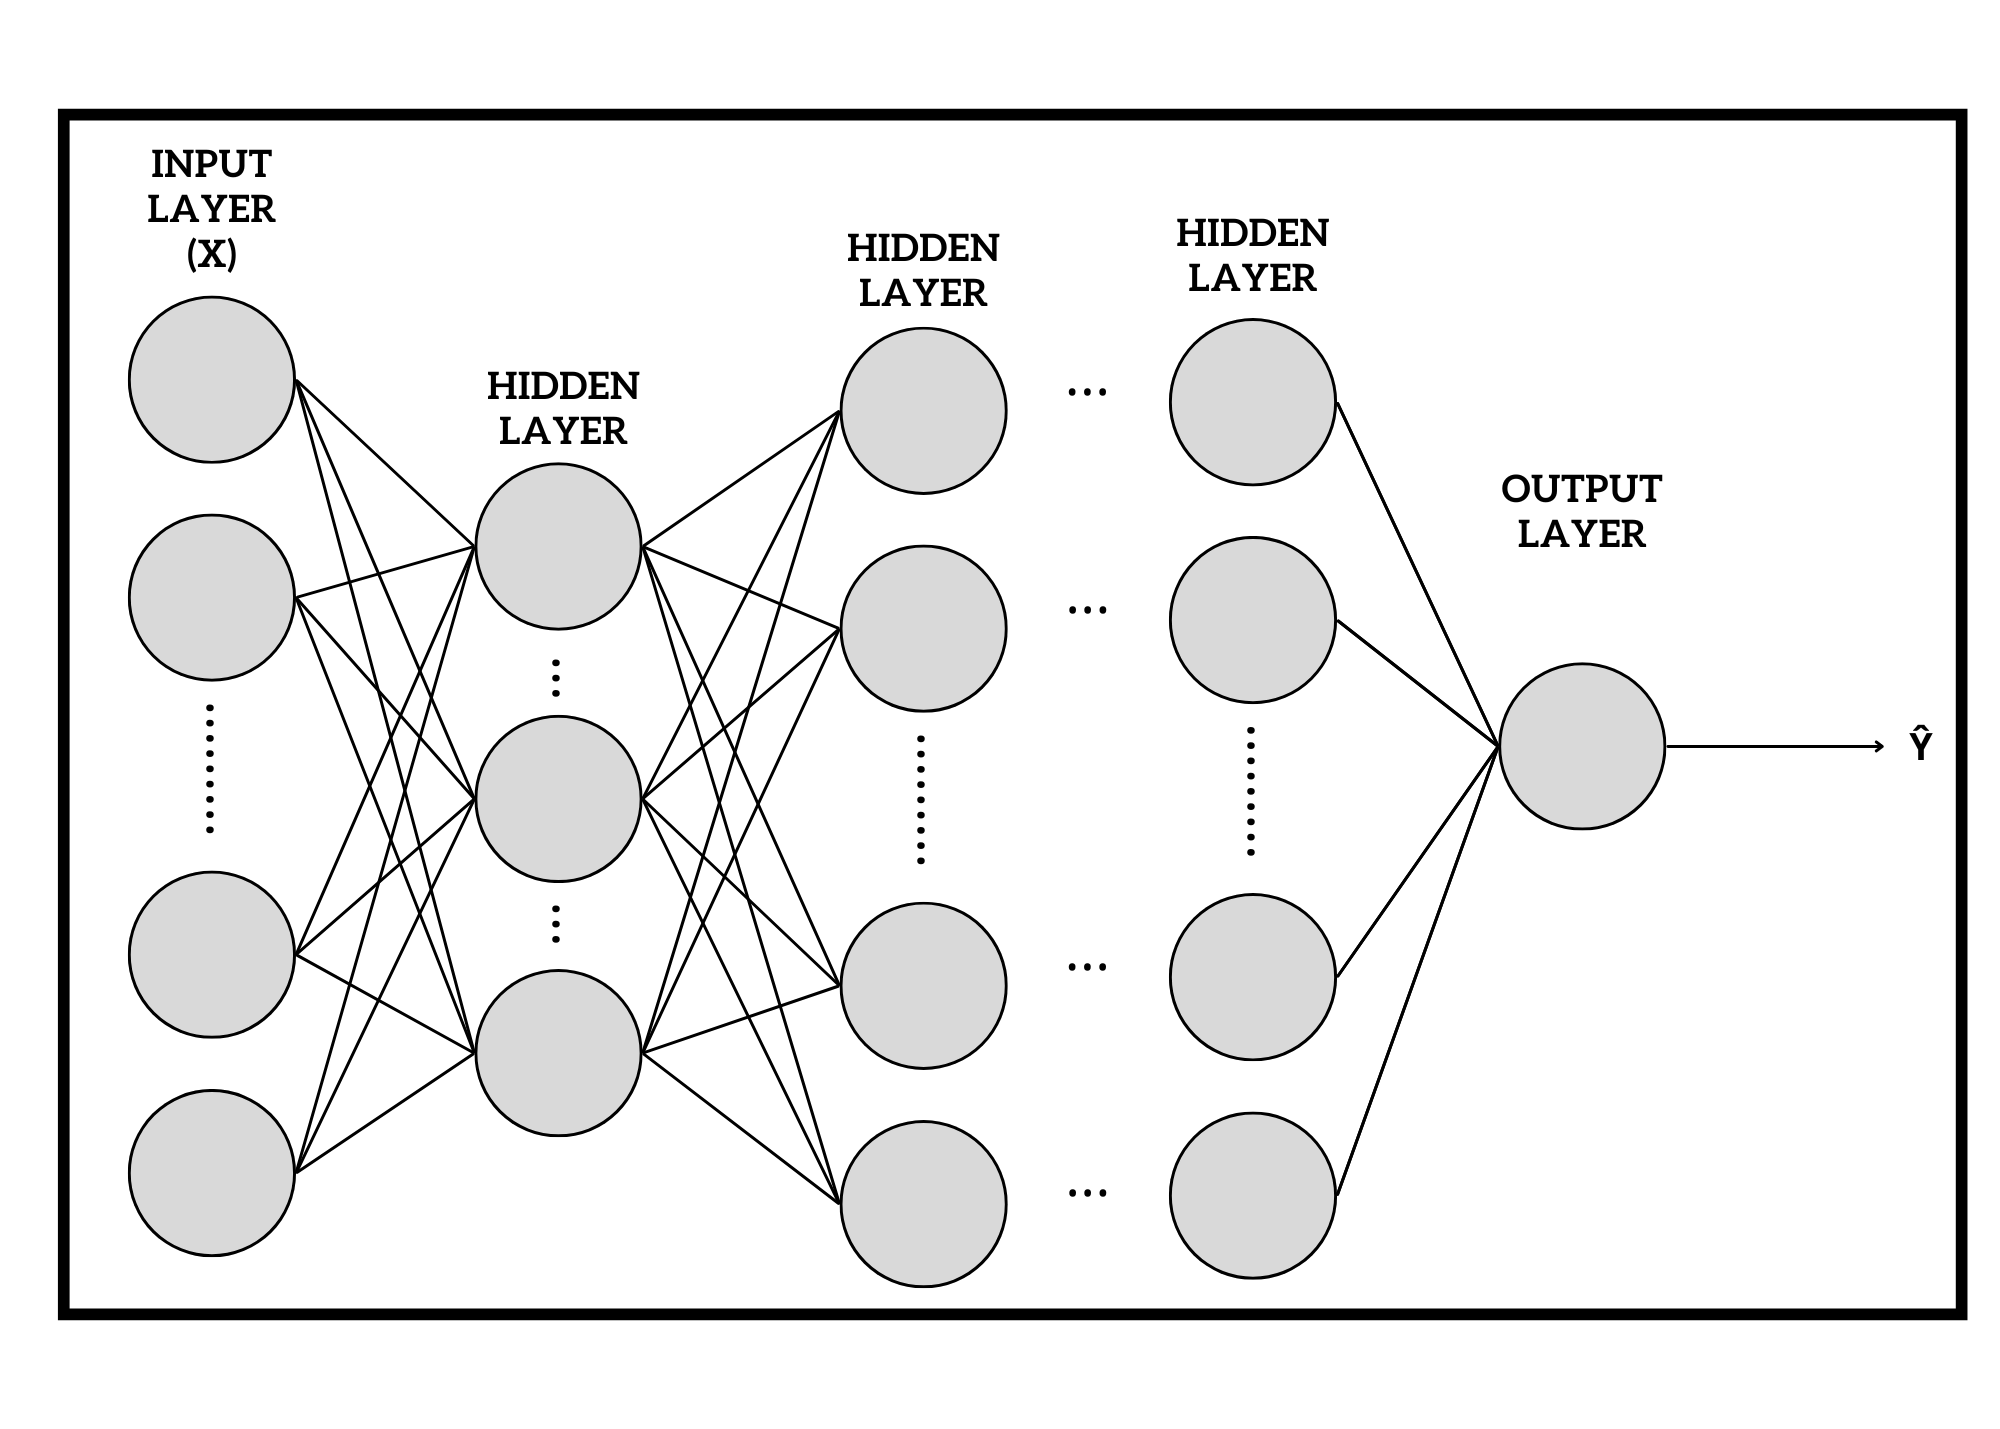
\includegraphics[width=0.8\textwidth]{Neural Network.png}
  \caption{Structure behind Supervised-Learning based Neural Network}
\end{figure}

Each node in the input layer contains a distinct feature. The total amount of features considered is 13 using the Heart Disease database offered by the University of California, Irvine.

\textbf{Feature Listing}

\begin{itemize}
    \item Age
    \item Sex
    \item cp: Chest pain type
    \begin{itemize}
        \item Value 1: Typical Angina
        \item Value 2: Atypical Angina
        \item Value 3: Non-anginal pain
        \item Value 4: Asymptomatic
    \end{itemize}
    \item trestbps: Resting blood pressure in mm Hg on admission to the hospital
    \item fbs: (Fasting blood sugar $> 120$ mg/dl) (1 = true; 0 = false)
    \item restecg: Resting electrocardiographic results:
    \begin{itemize}
        \item Value 0: Normal
        \item Value 1: Having ST-T wave abnormality (T wave inversions and/or ST elevation or depression of $> 0.05$ mV)
        \item Value 2: Showing probable or definite left ventricular hypertrophy by Estes' criteria
    \end{itemize}
    \item thalach: Maximum heart rate achieved
    \item exang: Exercise induced angina (1 = yes; 0 = no)
    \item oldpeak: ST depression induced by exercise relative to rest
    \item slope: The slope of the peak exercise ST segment
    \begin{itemize}
        \item Value 1: Upsloping
        \item Value 2: Flat
        \item Value 3: Downsloping
    \end{itemize}
    \item ca: Number of major vessels $(0-3)$ colored by fluoroscopy
    \item thal: 3 = normal; 6 = fixed defect; 7 = reversible defect
\end{itemize}

And the target considered is the presence = 1 or absence = 0 of heart disease in the variable "num".

\textbf{Input Layer Interpretation}

To examplify what occurs in the nodes in the input layer, in this dataframe, each row is a sample that contains 13 elements/features. Consider three samples as vectors:
\begin{equation}
    \begin{aligned}
    s_{1} &= \langle v_{1,1}, v_{1,2}, \ldots, v_{1,13} \rangle \\
    s_{2} &= \langle v_{2,1}, v_{2,2}, \ldots, v_{2,13} \rangle \\
    s_{3} &= \langle v_{3,1}, v_{3,2}, \ldots, v_{3,13} \rangle
    \end{aligned}
\end{equation}

One node will be composed of \( x_{1} = \langle v_{1,1}, v_{2,1}, v_{3,1} \rangle \), the next one of \( x_{2} = \langle v_{1,2}, v_{2,2}, v_{3,2} \rangle \), and so on for a generalized case with more samples. This means that each node contains one feature collected from the given samples.

\textbf{Data Processing}

All the samples with missing values have been dropped from the analysis, the samples have been shuffled randomly, and 80\% of the data (samples) has been assigned to training \( (X_{\text{train}}, y_{\text{train}}) \) and 20\% to testing \( (X_{\text{test}}, y_{\text{test}}) \), where \( X \) is the set of input features and \( y \) is the set of target values.
After, all the input values were normalized. The process ocurred by dividing all the values from a given feature by the maximum number found on the same feature.

Then, standarization was applied to ensure that all features contribute equally to the model which is defined by

\begin{equation}
    t = \frac{x-\mu}{\sigma}
\end{equation}
where $x$: original input value, $\mu$: mean of input values, $\sigma$: Standard deviation of the feature values, $t$: Standarized value such that $n$ is the number of values in $X_{train}$ and
\begin{equation}
    \mu = \frac{1}{n}\sum_{i = 1}^{n}x_{i}
\end{equation}

\begin{equation}
    \sigma = \sqrt{\frac{1}{n}\sum_{i = 1}^{n}(x_{i}-\mu)^2}
\end{equation}

On the other hand, $X_{test}$ is standarized by using the mean and standard deviation of $X_{train}$ to guarantee the model evaluates new data in the same way than when evaluating training data which avoids overfitting.



\textbf{Forward Propagation}\\
The way to compute the values of the neurons in the first layer (the one after the input layer) is the following:
% Z = 10x13, W = 10x297, A = 297x13, b = 10x13 
\[
\begin{bmatrix}
   z_{1,1} & \cdots & z_{1,13} \\
   z_{2,1} & \cdots & z_{2,13} \\
   \vdots &   & \vdots \\
   z_{11,1} & \cdots & z_{11,13}
\end{bmatrix}
=
\begin{bmatrix}
    w_{1,1} & \cdots & w_{1,297} \\
    w_{2,1} & \cdots & w_{2,297} \\
    \vdots &   & \vdots \\
    w_{11,1} & \cdots & w_{11,297}
\end{bmatrix}
\begin{bmatrix}
    x_{1,1} & \cdots & x_{1,13} \\
    x_{2,1} & \cdots & x_{2,13} \\
    \vdots &   & \vdots \\
    x_{297,1} & \cdots & x_{297,13}
\end{bmatrix}
+
\begin{bmatrix}
    b_{1,1} & \cdots & b_{1,13} \\
    b_{2,1} & \cdots & b_{2,13} \\
    \vdots &   & \vdots \\
    b_{11,1} & \cdots & b_{11,13}
\end{bmatrix}
\]

Which can be re-writed as 

\begin{equation}
    Z^{[1]} = W^{[1]}X^{[0]} + B^{[1]} := Layer \quad 1
\end{equation}

Such that each row in $Z$ represents the information contained in a neuron of the first layer.
% Important: The activation functions for hidden and output layers are subject to change, as well as the shape in the input dataset, and the number of layers and neurons
The new matrix $Z$ becomes the input for an activation function, which in this case is the Rectified Linear Unit (ReLU). The activation function is necessary because it allows us to approximate non-linear functions, which implies that ReLU has to be non-linear,
and it is defined in the following manner:
\[
ReLU(x) = 
\begin{cases} 
   x & \text{if } x > 0 \\
    0 & \text{if } x \leq 0 \\
\end{cases}
\]
Now all the values in $Z$ are input in ReLU which defines a new matrix:

\begin{equation}
    A^{[1]} = ReLU(Z^{[1]})
\end{equation}
To get the values of the second layer we use $A^{[1]}$ as its input in the same way that it was done before:
\begin{equation}
    Z^{[2]} = W^{[2]}A^{[1]} + B^{[2]} := Layer \quad 2
\end{equation}
Where, as before, the number of rows in $Z$ is the number of neurons in that layer, and its number of columns is the number of features used in the model which is 13. The shape of $A^{[1]}$ is the same as that of $Z^{[2]}$.
The shape of $W$ is determined equally as before: the number of rows is the number of neurons in the new layer and its  number of columns is the amount of rows of the matrix it is multiplied to ($A^{[1]}$). Ultimately, the shape of $B^{[1]}$ is one such that the number of rows is equal to the number of neurons in the new layer and its number of columns is equal to the number of columns of the ``input matrix" which previously was $X^{[0]}$ but now is $A^{[1]}$.\\

The mentioned process is iterated for the rest of the layers until the output layer which consists of only one neuron. Which means that the equation for the hidden layer would be
\begin{equation}
    Output = W^{[n]} \cdot A^{[n-1]} + B^{[n]} = \langle w_{1}, w_{2}, \ldots , w_{13} \rangle \cdot \langle a_{1}, a_{2}, \ldots , a_{13} \rangle + b
\end{equation}
Which implies that
\begin{equation}
    Output = w_{1}a_{1} + \cdots + w_{13}a_{13} + b
\end{equation}

At that point a different activation function is used which is called Sigmoid. This function is defined in the following manner:

\[
Sigmoid\,(z) = \frac{1}{1+e^{-z}}
\]

Which is incredibly useful because Sigmoid$\,(x) \in (0,1) \quad \forall x \in (-\infty,\infty)$ which means that we can express the scalar obtained in the output layer in a value between 0 and 1. 
The latter provides a probabilistic interpretation of the results, the value obtained from Sigmoid can be rounded to 1 or 0 meaning that $y$ predicted would be acquired after that process. Remember that $y$ is our target which is presence or absence of heart disease.
Therefore,

\[
\hat{Y} = 
\begin{cases} 
   1 & \text{if } \text{Sigmoid}(z) \geq 0.5 \\
   0 & \text{if } \text{Sigmoid}(z) < 0.5 \\
\end{cases}
\]

\underline{Important remark}: All the weights $(w)$ and biases $(b)$ are initially picked randomly but are later adjusted properly in a process called Backpropagation to improve predictions\\
% If the number of features is changed re-check this part
\textbf{Loss Function}\\
We need to measure the quality of the model so that, afterwards, parameters could be readjusted to find the desired results during the training stage in supervised learning.
The function selected to determine accuracy is the Binary Cross Entropy Loss Function (BCE) which is calculated in the following manner
\begin{equation}
    BCE = -\frac{1}{N}\sum_{i = 0}^{N}[y_ilog(\hat{y}_i)+(1-y_i)log(1-\hat{y}_i)]
\end{equation}
Where $y_i$ is the actual target (0 or 1), $\hat{y}_i$ is the predicted probability of the target (not yet rounded), and $N$ is the number of samples.

It is useful because it is a binary classifier and the model has as targets 0 or 1, and penalizes confident but incorrect predictions.

Since the numeric values inside of the logarithms are between 0 and 1 the logarithms are negative or 0. Therefore, the negative sign that affects the whole sum serves to make $BCE$ positive.

\textbf{Backpropagation}

The idea is to minize the loss function. That is to minimize inaccuracies in the model. To do this we have to remember that we selected random values as weights and biases
but these could have been just defined in terms of variables. If we apply all the process and do not select any set of numbers for weights and biases ultimately, we would have the BCE expressed in terms of these unknowns too.

\textbf{Stochastic Gradient Descend}

We need to determine the ``level of influence'' that the weights and intercepts have on the Loss Function. And we can do it by Partial Derivatives and the Chain Rule. Consider that $W$ and $B$ are matrices of the containing $w_1, w_2, ... $ and $b_1, b_2, ... $ respectively but in this case as variables not numerical values.
\begin{equation}
    \frac{\partial BCE}{\partial W} = \frac{\partial BCE}{\partial \hat{y}} \cdot \frac{\partial \hat{y}}{\partial W}
\end{equation}

\begin{equation}
    \frac{\partial BCE}{\partial B} = \frac{\partial BCE}{\partial \hat{y}} \cdot \frac{\partial \hat{y}}{\partial B}
\end{equation}
Consider that now $\hat{y}$ is the function of the model without being rounded.

Now, after acquiring
\begin{equation}
    \frac{\partial BCE}{\partial W}
\end{equation}
and
\begin{equation}
    \frac{\partial BCE}{\partial B}
\end{equation}
We can plug in each weight and bias that was initially selected randomly into these functions. We would have

\begin{equation}
    \frac{\partial BCE}{\partial W} (W^{[1]}) \quad \wedge \quad \frac{\partial BCE}{\partial B} (B^{[1]})
\end{equation}

Now we can finally update our parameters in order to get a better prediction. We can begin minimizing the Loss Function by getting the derivative close to 0.
So we can ``move'' in the loss function to get closer to the global or local minimum by steps (remember that the matrix $X$ has fixed values). This step size is called in Machine Learning lingo as learning rate.

% This applies when the function is of degree 2, we need to analyze how to get to the minimum in this new loss function

Therefore, we can define step sizes in the following manner:

\begin{equation}
    Step \, \, Size_W = \alpha \, \, \frac{\partial BCE}{\partial W} (W^{[1]})
\end{equation}
\begin{equation}
    Step \, \, Size_B = \alpha \, \, \frac{\partial BCE}{\partial B} (B^{[1]})
\end{equation}
And now we can update the original random parameters selected in $W^{[1]}$ and $B^{[1]}$ in the following way

\begin{equation}
    New \, \, W^{[1]} = W^{[1]} - Step \, \, Size_W
\end{equation}
\begin{equation}
    New \, \, B^{[1]} = B^{[1]} - Step \, \, Size_B
\end{equation}

And with this we are done with one epoch (interation which begins with input weights and biases and is concluded with the re-update of weights and biases).
We model can go through thousands of epochs without problems and have a much more perfect prediction of targets.

But consider that this process (Gradient Descend) is slow for big data. So we use Stochastic Gradient Descend (SGD) which accelerates the process. SGD uses the
name algorithm that was described but uses the points that determine the Loss Function differently (the Loss Function can be graphed in a 3D Cartesian Plane with axes ``weight'', ``bias'' and BCE). That is, it updates the weights and biases using only one randomly selected data point at a time and
introduces noise into the parameters updates which lead to higher variance in the updates.

It is reasonable to ask ourselves: Until when does Stochastic Gradient Descend stop? and the answer is until the number of epochs precised to the model is completed.

\textbf{Important Remark}: In this neural network each layer has its own random weights and biases at the beginning (that's why they are expressed in distinct matrices). So, per epoch not just the first weights and biases get updated but all of them in the different layers.

% There are additional reasons for which it would be better to stop SGD or continue with SGD

\textbf{Code}

\lstinputlisting[language=Python, caption= Cardiovascular Diseases Diagnosis Predictor label=code:python_example_file]{Cardiovascular Diseases Diagnosis Predictor - Copy.py}

\subsection*{Neural Network for Treatment}
\subsection*{K-Nearest Neighbours Algorithm for Imaging Interpretation}
To analyze any set of pictures derived from medical imaging consider a 3D graph with axes Red, Green, and Blue (RGB).
\begin{center}
    \begin{tikzpicture}
        \begin{axis}[
            view={60}{30},
            axis lines=center,
            xlabel={\textcolor{red}{Red}},
            ylabel={\textcolor{darkgreen}{Green}},
            zlabel={\textcolor{blue}{Blue}},
            xmax=255, xmin=0,
            ymax=255, ymin=0,
            zmax=255, zmin=0,
            xtick={0, 255},
            ytick={0, 255},
            ztick={0, 255},
            colormap name=viridis,
        ]
        \end{axis}
        \node at (0, 1.3) {0};
    \end{tikzpicture}
\end{center}
\begin{center}
    \textbf{Figure 2:} 3D Cartesian Coordinate System with RGB-Labeled Axes
\end{center}
Each pixel in an image is going to contain a 3-tuple that represents it in the form of RGB with numbers ranging from 0 to 255. Therefore, a RGB coordinate can be expressed in the
presented graph as (red value, green value, blue value). Each picture is going to have a set of pixels that have their respective coordinates. That will generate many clusters of points
such that each cluster represents an image. Let's image, we have three images and each dot in the next graph represents the RGB code of a pixel:

\begin{figure}[h]
    \centering
    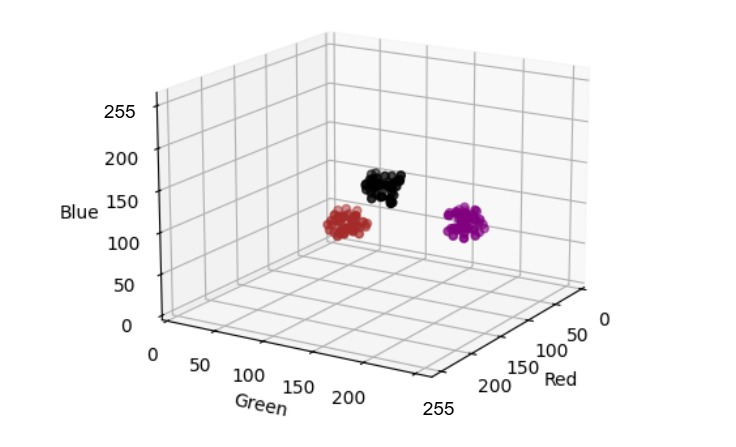
\includegraphics[width=0.7\textwidth]{WhatsApp Image 2024-07-05 at 4.24.08 PM.jpeg}
\end{figure}
\begin{center}
    \textbf{Figure 3:} Presence of Clusters to Illustrate Imaging Graphical Interpretation
\end{center}

\textbf{Important Remark}: The colors in the dots (black, purple, and orange) are just a way to emphasize the distinctiveness among clusters. They do not have any additional interpretational value.

Considering Fig. 3, where all the dots already present were part of the training dataset, we would like to provide a new and unseen dot to see how the model predicts to which cluster is belongs.

\begin{figure}[h]
    \centering
    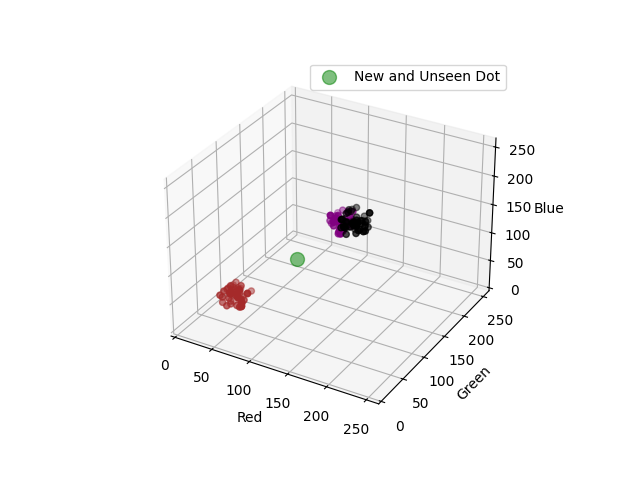
\includegraphics[width=0.45\textwidth]{Figure_1.png}
  \end{figure}
  \begin{center}
    \textbf{Figure 4:} Addition of unseen datapoint
\end{center}

What the K-Nearest Neighbours algorithm does it that it measures the distance of this unseen datapoint with respect to the other points in the training dataset, observes the ``k'' points (which, by the way, are labelled with respect to the cluster they belong to) that are the the closest to the new datapoint,
and performs a majority vote. That is, if for example the majority of the ``k'' points that are the closest to the new datapoint are labelled as ``Cluster 1'', then the new datapoint gets classified as belonging to ``Cluster 1''. Note that $k \in \mathbb{N}$   that could be used for instance as ``The 4 points that are the closest to the new data point'', where $ k = 4$

It is important to note that the distance between points will be calculated using the euclidian distance formula in the 3D Cartesian Plane which is the following:

\begin{equation}
    D=\sqrt{ (x_2-x_1)^2+ (y_2 -y_1)^2+ (z_2-z_1)^2}
\end{equation}

Where $x$ stands for the value of red, $y$ for that of green, and finally $z$ for that of blue.

This base model is very useful when we have sets of images that have very distinct colors, however, in the case of fMRI, for example, there are many times where similar colors are expressed but their combination as a whole is
what can generate a sudden and important change in diagnosis.

To account for the situation of similar color usage but relevance in differences in overall view, the following approach is proposed.

The new graph to consider would be an $n$-dimensional one, that means that each coordinate could belong to $\mathbb{R}^{n}$ such that $n$ is a multiple of 3.
Each datapoint will be expressed as a datapoint in the following manner:

\begin{equation}
    (Rv_{1},Gv_{1},Bv{1},Rv_{2},Gv_{2},Bv{2},\ldots,Rv_{p},Gv_{p},Bv{p})
\end{equation}

Where $p$ stands for the number of pixels in the image. The way pixels are numbered is from left to right from top to bottom.

Through this approach, each image in the training dataset would contain all the color information about all their pixeles in ordered manner generating a more precise learning outcome for the model.

The euclidian formula of distance now applied to an $n$ dimensional space would be the following:

\begin{equation}
    \sqrt{(u_1-v_1)^2+(u_2-v_2)^2+\cdots+(u_n-v_n)^2}
\end{equation}

The mechanism of the K-Nearest Neighbours by considering clusters and majority vote would be the same but now applied to images instead of individual pixels to take into consideration the grand scheme of details.

\end{document}

